\section{Project Overview}

    Physical infrastructure is a large and complicated subject, encompassing everything from running water to mains electricity. Below I have listed the main features included in physical infrastructure:

    \begin{itemize}
        \item \textbf{Transportation:} Road and highway networks; Mass transit systems; Railways; Canals; Seaports; Airports; Bicycle paths / pedestrian walkways

        \item \textbf{Energy:} Electrical power network; Natural gas pipelines; Petroleum pipelines; Coal production and processing

        \item \textbf{Water management:} Drinking water supply; Sewage collection; Drainage systems; Irrigation systems; Flood control systems; Coastal management

        \item \textbf{Communications:} Postal service; Telephone networks; Mobile phone networks; Television and radio stations; Internet services; Communications satellites; Undersea cables

        \item \textbf{Solid waste management:} Landfills; Incinerators; Hazardous waste disposal
    \end{itemize}

    Computer modelling systems could be developed for any one of these areas, allowing users to prototype infrastructure designs before the costly process of constructing it. For this project I have chosen to focus on the Transportation sector, as it can include some of the most expensive forms of infrastructure.

    Naturally the major responsibility of transportation infrastructure goes towards the construction and maintenance of road networks, including but not limited to junctions, roundabouts, highways and traffic lights.
    These networks can get very complicated and difficult to manage, for example the UK's so called "spaghetti junction" in Birmingham.

    \begin{figure}[h]
        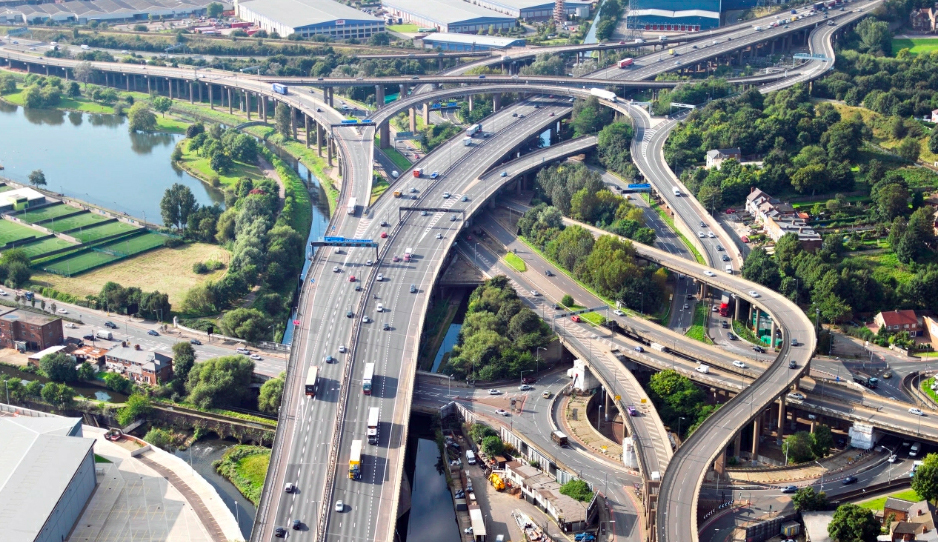
\includegraphics[width=0.5\textwidth]{Spaghetti-Junction.jpg}
        \centering
        \caption{Birmingham's "Spaghetti junction" \cite{Spaghetti-Junction}}
    \end{figure}

\section{The Problem}

    Development of transportation is a very expensive and time consuming process, so being able to evaluate the efficiency and cost-effectiveness of road layouts beforehand would be very beneficial. This project aims to develop a road network simulator that can be used to evaluate the efficiency of inputted designs under a range of different traffic conditions.

    \subsection{End user}

\section{Current Systems}

    \subsection{AnyLogic - Road Traffic Simulation Software}

        AnyLogic - Road Traffic Simulation Software \cite{AnyLogic} is an industry-level program used for analysing traffic patterns and behaviours, below are a couple images of the program.

        \begin{figure}[ht]
            \centering
            \begin{minipage}{0.3\textwidth}
                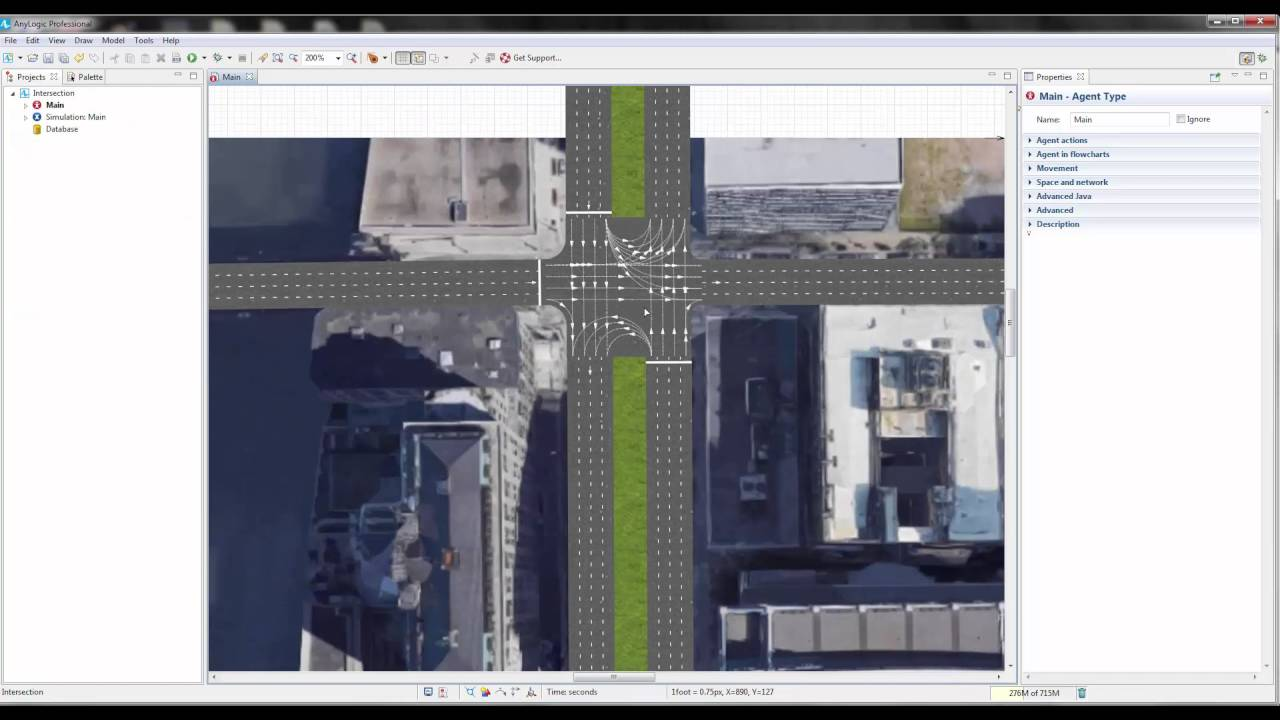
\includegraphics[width=0.8\textwidth]{anylogic-image-1.jpg}
                \caption{Happy Smiley}
            \end{minipage}
            \begin{minipage}{0.3\textwidth}
                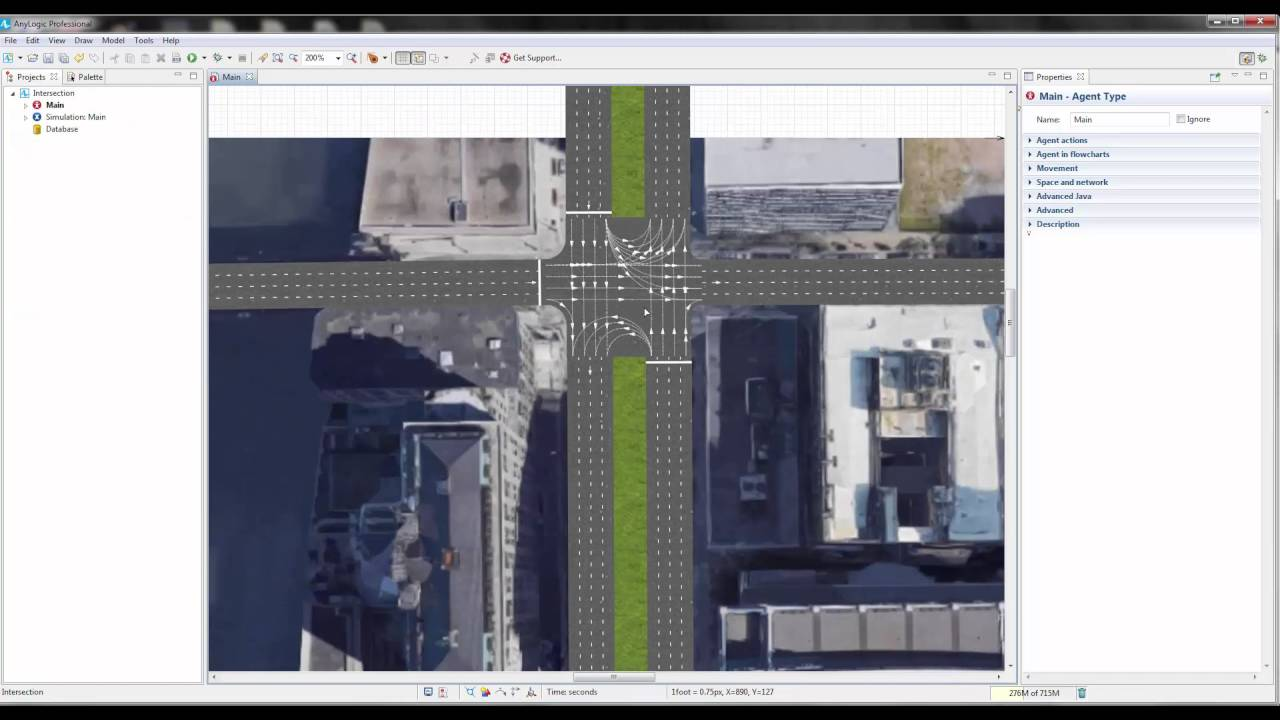
\includegraphics[width=0.8\textwidth]{anylogic-image-1.jpg}
                \caption{Sad Smiley}
            \end{minipage}
            \begin{minipage}{0.3\textwidth}
                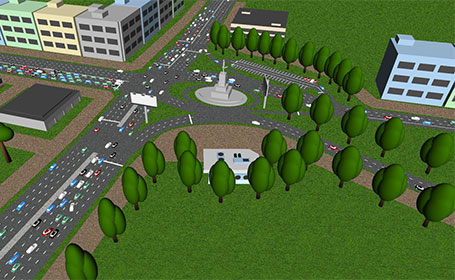
\includegraphics[width=0.8\textwidth]{anylogic-image-3.jpg}
                \caption{Sad Smiley}
            \end{minipage}
        \end{figure}

    \subsection{SOUND}

    \subsection{Eclipse SUMO}

\section{Research}

    \subsection{Traffic laws}

        This project will be based off the UK Highway Code \cite{Highway-Code} as of the latest update (23 March 2021). This document contains all laws and regulations for driving in the UK. The relevant points include:

        \begin{itemize}
            \item Normal driving position is considered the leftmost lane of the road and should be assumed whenever possible
            \item Right-of-way is given to the major road when emerging from a junction
            \item When entering a roundabout, you must give way to vehicles on your right
            \item Is it recommended to maintain a two second separation distance from the vehicle in front
        \end{itemize}

        These rules will be used to inform how the vehicles in the simulation operate in different circumstances. Although it may be noted that not all vehicles follow these laws strictly, so deviations may be added to account for this.

    \subsection{Graphs}

        The natural way to represent any kind of network (including road networks) programmatically is using a graph, so I will conduct some preliminary research into this topic.

        Graphs are an abstract data structure used to describe a set of vertices and the edges connecting them, both vertices and edges can have associated values. This is a very useful structure in computer science as it can be used to model a wide range of existing data such as power grids and social networks. Graphs also come with a wide range of existing algorithms for operating on them such as Dijkstra's shortest path algorithm or the A* search algorithm.

        Described below are the two most common data structures used to describe graphs:

        \begin{itemize}
            \item \textbf{Adjacency list} - Vertices are stored as objects containing a list of it's own adjacent vertices.
            \item \textbf{Adjacency matrix} - A two-dimensional matrix where each cell represents the edge (or lack of edge) from the vertex described by the row to the vertex described by the column.
        \end{itemize}

        Each implementation has its advantages and disadvantages \autoref{graph-time-complexities} shows the time complexity of each operation over these two structures.


        \begin{table}[h]
            \centering
            \begin{tabular}{|p{0.2\linewidth}|p{0.2\linewidth}|p{0.2\linewidth}|} \hline
            & Adjacency list & Adjacency matrix \\ \hline
            Store graph   & $O(|V|+|E|)$ & $O(|V|^2)$ \\ \hline
            Add vertex    & $O(1)$ & $O(|V|^2)$ \\ \hline
            Add edge      & $O(1)$ & $O(1)$ \\ \hline
            Remove vertex & $O(|E|)$ & $O(|V|^2)$ \\ \hline
            Remove edge   & $O(|V|)$ & $O(1)$ \\ \hline
            Check for adjacency between two vertices & $O(|V|)$ & $O(1)$ \\ \hline
            \end{tabular}
            \caption{Time complexities of different graph implementations \cite{graph-time-complexities}}
            \label{graph-time-complexities}
        \end{table}

        Since road networks are generally optimised for maximum throughput I will also research the graph maximum flow problem as this may be useful in evaluating the networks. Formally, the maximum flow problem is as follows \cite{citation needed}:

        \begin{itemize}
            \item Let $N = (V,E)$ be a network with $s, t \in V$, where $s$ is the source and $t$ is the sink.
            \item The capacity of an edge is the maximum flow that can pass through it, the capacity from vertex $v$ to vertex $u$ is denoted as $c_{uv}$; and flow on the same edge as $f_{uv}$.
            \item The flow network must satisfy two properties:
            \begin{itemize}
                \item Capacity constraint: The flow of an edge cannot exceed it's capacity. \[\forall (u, v) \in E : f_{uv} \leq c_{uv}\]
                \item Conservation constraint: The flow into a vertex must equal the flow exiting a vertex (the source and sink are exceptions).
                \[\forall v \in V \setminus \{s, t\} : \sum_{u : (u, v) \in E} f_{uv} = \sum_{u : (v, u) \in E} f_{vu}\]
            \end{itemize}
            \item The value of flow is the total amount of flow passing from the source to the sink, given by:
            \[|f| = \sum_{v : (s, v) \in E} f_{sv}\]
        \end{itemize}

        The goal of the maximum flow problem is to route as much flow as possible from the source to the sink under these constraints. Many algorithms to compute $f_\text{max}$ have been found including but not limited to Linear Programming, the Ford-Fulkerson algorithm or the Edmonds-Karp algorithm.

        The maximum flow of a road network could be a good indicator of the theoretical maximum efficiency.

\section{Proposed Solution}

    My proposed solution consists of a desktop app that allows the user to construct an arbitrary road network and test it using a set of 'car' agents that traverse the network.

\section{Objectives}
